%++++++++++++++++++++++++++++++++++++++++
\documentclass[letterpaper,12pt]{article}
\usepackage[square,numbers]{natbib}
\bibliographystyle{unsrtnat}
\usepackage{placeins}
\usepackage{tabularx}
\usepackage{amsmath}
\usepackage{amssymb}
\usepackage{graphicx}
\usepackage[margin=1in,letterpaper]{geometry}
\usepackage[final]{hyperref}
\usepackage{float}
\usepackage{multirow}
\usepackage{listings}
\usepackage{tikz}
\usetikzlibrary{positioning,arrows.meta,calc}
\lstset{basicstyle=\footnotesize\ttfamily, breaklines=true, breakatwhitespace=true}
\usepackage[skip=-1pt]{caption}
\usepackage{enumitem}
\hypersetup{colorlinks=true,linkcolor=black,citecolor=black,filecolor=black,urlcolor=black}
%++++++++++++++++++++++++++++++++++++++++

\begin{document}
\pagenumbering{none}
\begin{figure}
    \centering
    \includegraphics[width=0.8\linewidth]{logo.png}
    \label{fig:placeholder}
\end{figure}

\begin{center}
    \textbf{\Large Fixed-Point MAC Unit for Neural Inference}\\[4pt]
    \large A parameterised signed multiply-accumulate unit in Verilog-2001
\end{center}

\vspace{1cm}

\renewcommand{\arraystretch}{1.5}
\setlength{\tabcolsep}{10pt}

\begin{tabular}{|p{5cm}|p{9cm}|}
\hline
Name & Pierre Kostantine \\\hline
Student ID & 501285659 \\\hline
Date & September 16, 2026 \\\hline
Repository & \url{https://github.com/pKostantine/mac-unit} \\\hline
Targets & Lattice iCE40HX1K-VQ100, AMD Artix-7 XC7A35T-1L \\\hline
\end{tabular}

\newpage
\pagenumbering{roman}
\tableofcontents

\newpage
\pagenumbering{arabic}

%-----------------------------------------------------------
\section{Introduction: The MAC as the Unit of Inference}
%-----------------------------------------------------------

The multiply-accumulate (MAC) operation is the atomic unit of neural network
inference. A dense layer, a convolution and a matrix multiply are all
collections of dot products, and a dot product is a sequence of MACs. A
hardware inference engine is therefore, to first order, an arrangement of MAC
units and the memory bandwidth to feed them, which makes the cost of a single
MAC the number that determines how much of a network fits on a given die.

This project designs, verifies and characterises one such unit in
Verilog-2001: a parameterised signed fixed-point MAC with quantized (Q1.7)
operands, round-to-nearest output scaling, a saturating output path and sticky
accumulator overflow detection. The design is deliberately restricted to
Verilog-2001 so that the same source synthesises unchanged in Lattice
iCEcube2, AMD Vivado, Intel Quartus and the open-source Yosys flow.

The work is organised around a single question that the arithmetic alone does
not answer: \emph{what does numerical correctness cost in silicon?} The unit is
synthesised and timing-closed on two parts of different vendors, process nodes
and architectures, run on real hardware, and then deliberately stripped down in
order to measure the area and frequency price of the overflow, rounding and
saturation logic that surrounds the multiply-accumulate itself.

%-----------------------------------------------------------
\section{Objectives}
%-----------------------------------------------------------

The unit was required to satisfy the following:

\begin{itemize}
    \item One signed multiply-accumulate per clock cycle while enabled
    \item Parameterised operand width, accumulator width and fractional bit count, with no value hardcoded in the datapath
    \item Full-precision internal accumulation, with a guard band sized for realistic layer depth
    \item Round-to-nearest, rather than truncation, on the scaled output
    \item Saturating output rather than wraparound
    \item Sticky detection of accumulator overflow, surviving until cleared
    \item Synchronous \texttt{clear} outranking \texttt{enable}; asynchronous active-low reset outranking both
    \item Verilog-2001 only, for cross-vendor portability
    \item Verified by a self-checking testbench against an independent golden model
    \item Demonstrated on physical hardware, not simulation alone
\end{itemize}

%-----------------------------------------------------------
\section{Design Approach}
%-----------------------------------------------------------

The datapath is shown in Figure~\ref{fig:datapath}. Two signed
\texttt{WIDTH}-bit operands are multiplied to a $2\times$\texttt{WIDTH}-bit
product, accumulated into an \texttt{ACC\_WIDTH}-bit register, and the
accumulator is then scaled, range-checked and clamped to produce a
\texttt{WIDTH}-bit output. Three parameters control the whole structure:

\begin{itemize}
    \item \texttt{WIDTH} --- operand width, signed (default 8)
    \item \texttt{ACC\_WIDTH} --- accumulator width, signed (default 32)
    \item \texttt{FRAC\_BITS} --- fractional bits per operand (default 7, i.e.\ Q1.7)
\end{itemize}

\begin{figure}[H]
\centering
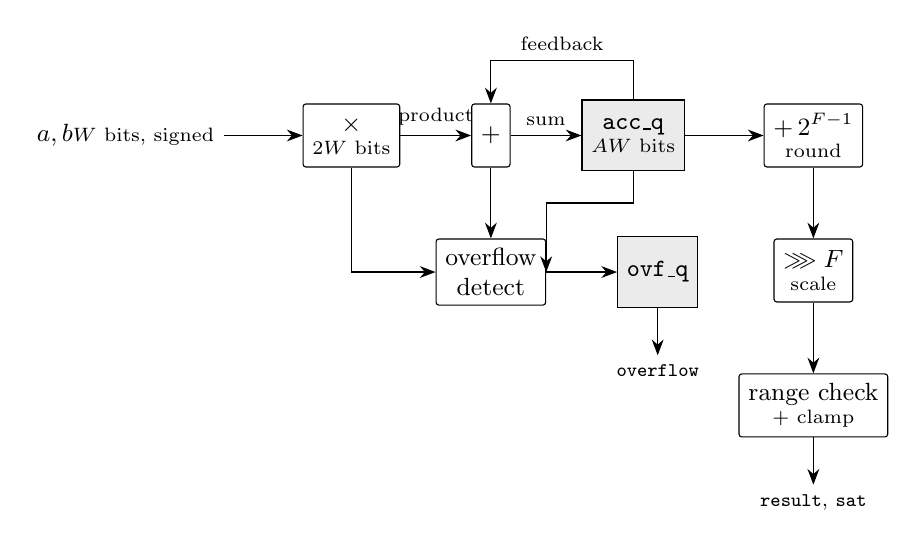
\begin{tikzpicture}[
    node distance=6mm,
    box/.style={draw, rounded corners=1pt, minimum height=8mm, align=center, font=\small},
    reg/.style={draw, fill=black!8, minimum height=9mm, align=center, font=\small},
    >={Stealth[length=2mm]}
]
\node[box] (mul) {$\times$\\[-1mm]\scriptsize $2W$ bits};
\node[left=10mm of mul, font=\small] (ab) {$a,b$\\[-1mm]\scriptsize $W$ bits, signed};
\node[box, right=9mm of mul] (add) {$+$};
\node[reg, right=9mm of add] (accq) {\texttt{acc\_q}\\[-1mm]\scriptsize $AW$ bits};
\node[box, below=9mm of add, font=\small] (ovf) {overflow\\detect};
\node[reg, right=9mm of ovf] (ovfq) {\texttt{ovf\_q}};
\node[box, right=10mm of accq] (rnd) {$+\,2^{F-1}$\\[-1mm]\scriptsize round};
\node[box, below=9mm of rnd] (shr) {$\ggg F$\\[-1mm]\scriptsize scale};
\node[box, below=9mm of shr] (sat) {range check\\[-1mm]\scriptsize + clamp};

\draw[->] (ab) -- (mul);
\draw[->] (mul) -- node[above,font=\scriptsize]{product} (add);
\draw[->] (add) -- node[above,font=\scriptsize]{sum} (accq);
\draw[->] (mul.south) |- (ovf.west);
\draw[->] (add.south) -- (ovf.north);
\draw[->] (ovf) -- (ovfq);
\draw[->] (accq) -- (rnd);
\draw[->] (rnd) -- (shr);
\draw[->] (shr) -- (sat);
\draw[->] (sat.south) -- ++(0,-6mm) node[below,font=\scriptsize]{\texttt{result}, \texttt{sat}};
\draw[->] (ovfq.south) -- ++(0,-6mm) node[below,font=\scriptsize]{\texttt{overflow}};

% feedback
\draw[->] (accq.north) -- ++(0,5mm) -| node[pos=0.25,above,font=\scriptsize]{feedback} (add.north);
\draw[->] (accq.south) -- ++(0,-4mm) -| (ovf.east);
\end{tikzpicture}
\caption{MAC datapath. The accumulator feeds back into the adder; the shaded blocks are the only registers. The overflow detector taps \texttt{sum} before the register, which becomes significant in Section~\ref{sec:dsp}.}
\label{fig:datapath}
\end{figure}

\subsection{Control Priority}

The accumulator register implements a strict priority chain:

\begin{lstlisting}[language=Verilog]
always @(posedge clk or negedge rst_n) begin
    if (!rst_n)      begin acc_q <= 0; ovf_q <= 1'b0;        end
    else if (clear)  begin acc_q <= 0; ovf_q <= 1'b0;        end
    else if (en)     begin acc_q <= sum; ovf_q <= ovf_q | acc_ovf; end
end
\end{lstlisting}

\texttt{clear} must outrank \texttt{en} so that a running accumulator can be
zeroed without first being stalled. When neither is asserted the block assigns
nothing, which is what makes \texttt{acc\_q} hold its value; writing an
explicit \texttt{acc\_q <= acc\_q} branch would describe identical hardware but
obscure the intent.

%-----------------------------------------------------------
\section{Numerical Design for Quantized Inference}
%-----------------------------------------------------------

\subsection{Signedness}

Every operand in the datapath is declared \texttt{signed}. This is not
cosmetic. In Verilog, if any operand of an expression is unsigned, the entire
expression is evaluated as unsigned and sign extension silently fails ---
turning $-2$ into $254$ without any warning from the tool. A single missing
\texttt{signed} keyword anywhere in the chain corrupts every negative product.

\subsection{Bit Growth}

A signed $W\times W$ multiply requires exactly $2W$ bits. For $W = 8$ the
extreme products are
\[
(-128)\times(-128) = +16384, \qquad (-128)\times(+127) = -16256,
\]
both of which fit in signed 16 bits, and neither of which fits in 15.

\subsection{Accumulator Guard Band}

The accumulator is 32 bits against a 16-bit product, giving 16 bits of guard
band. The worst-case number of accumulations before overflow is
\[
N_{\max} = \frac{2^{\text{ACC\_WIDTH}-1}}{2^{2\cdot\text{WIDTH}-2}}
        = \frac{2^{31}}{2^{14}} = 2^{17} = 131{,}072 .
\]
A 1{,}024-input dense layer performs 1{,}024 MACs, so the default parameters
carry roughly $128\times$ headroom over a realistic layer. The guard band is
therefore not arbitrary: it is chosen against layer depth, and
\texttt{ACC\_WIDTH} is the parameter a designer would change when targeting
deeper layers.

\subsection{Q-Format and Rounding}

Q-format is an interpretation, not a circuit --- the multiplier is
bit-identical whatever \texttt{FRAC\_BITS} is set to. With Q1.7 inputs the
product is Q2.14 and the accumulator is Q18.14, so emitting a Q1.7 result
requires an arithmetic right shift by \texttt{FRAC\_BITS}.

The rounding term is what matters. Truncating a two's-complement value always
rounds toward $-\infty$, a constant $-0.5$~LSB bias. In a single operation this
is negligible; across a layer of hundreds of accumulations it compounds into a
systematic downward drift in every activation. Adding half an LSB before the
shift converts truncation into round-to-nearest:
\[
\texttt{rounded} = \texttt{acc\_q} + 2^{\text{FRAC\_BITS}-1}, \qquad
\texttt{scaled}  = \texttt{rounded} \ggg \text{FRAC\_BITS}.
\]

\subsection{Saturation}

A value fits in \texttt{WIDTH} signed bits exactly when every bit above the
sign position is a copy of the sign bit, so the range check reduces to testing
whether the top slice is all zeros or all ones:

\begin{lstlisting}[language=Verilog]
wire in_range = (scaled[AW-1:W-1] == {(AW-W+1){1'b0}}) ||
                (scaled[AW-1:W-1] == {(AW-W+1){1'b1}});
assign result = in_range ? scaled[W-1:0]
                         : (scaled[AW-1] ? RES_MIN : RES_MAX);
\end{lstlisting}

Saturating rather than wrapping is a correctness decision, not a stylistic one.
Wrapping turns an activation of $+1.2$ into $-0.8$ --- a sign flip that
propagates through every downstream layer. Clamping to $+127$ merely loses
magnitude. Every production DSP datapath saturates for this reason.

\subsection{Overflow Detection}

Signed addition can only overflow when both operands share a sign, and when it
does the result carries the opposite sign; adding numbers of opposite sign
always lands between them and cannot overflow. This gives a two-term test:

\begin{lstlisting}[language=Verilog]
wire acc_ovf = (acc_q[AW-1] == product[PW-1]) &&
               (sum[AW-1]   != acc_q[AW-1]);
\end{lstlisting}

The flag is sticky: once raised it survives until \texttt{clear} or reset, so a
transient overflow mid-layer cannot be missed by sampling at the wrong time.
Section~\ref{sec:critpath} shows that these three gates, which appear free in
the source, determine the maximum clock frequency on both target devices.

%-----------------------------------------------------------
\section{Verification}
%-----------------------------------------------------------

\subsection{Self-Checking Testbench}

Verification uses a self-checking testbench (\texttt{tb/tb\_mac.v}) built
around a 64-bit golden reference model computed independently of the RTL.
Every enabled cycle updates the model, and the model and the device under test
are compared on every check rather than on a final value, so the first
divergence is reported rather than the last.

\begin{table}[H]
\centering
\caption{Testbench coverage}
\label{tab:tb}
\renewcommand{\arraystretch}{1.3}
\begin{tabular}{|l|l|}
\hline
\textbf{Category} & \textbf{Cases} \\
\hline
Reset behaviour        & Asynchronous assert, accumulator and flag cleared \\
Arithmetic corners     & $\times 0$, $\times 1$, $-128\times-128$, $-128\times127$, $127\times127$ \\
Sign handling          & Mixed-sign operand sequences \\
Control priority       & \texttt{en} low holds, \texttt{clear} mid-sequence, \texttt{clear} beats \texttt{en} \\
Saturation             & Clamp high, clamp low, \texttt{sat} flag assertion \\
Accumulator overflow   & 140{,}000 worst-case accumulations, sticky flag, clear-deasserts \\
Randomised             & $2\times$ 5{,}000-MAC randomised sequences \\
\hline
\multicolumn{2}{|l|}{\textbf{16 tests, $\approx$150{,}074 checks per run}} \\
\hline
\end{tabular}
\end{table}

\subsection{Validating the Testbench by Mutation}

A passing testbench proves nothing unless the testbench can fail. Before the
results were trusted, the RTL was deliberately mutated --- inverting the
overflow comparison, removing the rounding term, replacing saturation with
truncation --- and each mutation was confirmed to produce failures. A
testbench that passes both the correct design and a broken one is measuring
nothing.

\subsection{Parameter Sweep}

\texttt{tb/tb\_param.v} is parameter-agnostic and was run across four
configurations. This caught a real defect: an early version of the output path
contained hardcoded constants (\texttt{32'sd64}, \texttt{>>> 7},
\texttt{[31:7]}) that happened to be correct at the default parameters. It
passed every test at 8/32/7 and failed everywhere else.

\begin{table}[H]
\centering
\caption{Parameter sweep, before and after the fix}
\label{tab:sweep}
\renewcommand{\arraystretch}{1.3}
\begin{tabular}{|l|c|c|}
\hline
\textbf{WIDTH / ACC\_WIDTH / FRAC\_BITS} & \textbf{Hardcoded version} & \textbf{Parameterised version} \\
\hline
8 / 32 / 7  & Pass          & Pass \\
4 / 16 / 3  & 8{,}212 errors & Pass \\
6 / 24 / 5  & 8{,}344 errors & Pass \\
12 / 40 / 9 & 5{,}327 errors & Pass \\
\hline
\end{tabular}
\end{table}

The lesson is that a module is not parameterised because its ports are
declared with parameters; it is parameterised when it has been tested at
parameters other than the default.

%-----------------------------------------------------------
\section{Synthesis Results}
%-----------------------------------------------------------

\subsection{Lattice iCE40HX1K --- iCEcube2 2020.12, Synplify Pro, post-route}

\begin{table}[H]
\centering
\caption{iCE40HX1K-VQ100 implementation results}
\label{tab:ice40}
\renewcommand{\arraystretch}{1.3}
\begin{tabular}{|l|c|}
\hline
\textbf{Metric} & \textbf{Value} \\
\hline
Maximum frequency (post-route) & \textbf{132.64 MHz} \\
Board clock                    & 25 MHz \\
Slack at 25 MHz                & $+32.46$ ns \\
Logic cells                    & 227 / 1280 (17.7\%) \\
\quad combinational            & 194 \\
\quad sequential               & 33 \\
LUT4s                          & 224 \\
Carry cells                    & 69 \\
Registers                      & 33 (32 accumulator + 1 sticky overflow) \\
Logic tiles (PLBs)             & 46 / 160 (28.8\%) \\
Block RAM                      & 0 / 16 \\
DSP blocks                     & none available on this part \\
I/O                            & 62 / 72 \\
\hline
\end{tabular}
\end{table}

The HX1K has no hard multipliers, so the entire multiply is built from LUT4s
and carry chains. At the Go Board's 25 MHz oscillator the design has $5.3\times$
frequency headroom, which means a pipelined variant is an optimisation
experiment for this board rather than a necessity.

Synthesis-time estimate was 85.3~MHz and post-placement 122.35~MHz, both
conservative against the 132.64~MHz post-route result. The post-route number is
the one quoted; the earlier two are estimates against modelled routing.

\subsection{AMD Artix-7 XC7A35T-1L --- Vivado 2026.1, post-route}

The same RTL was constrained at 5.000~ns (200~MHz) with the I/O declared false
paths, matching the treatment used on the iCE40, and run through synthesis,
placement and routing.

\begin{table}[H]
\centering
\caption{Artix-7 XC7A35T-1L (csg324) results, all post-route at 5.000 ns}
\label{tab:artix}
\renewcommand{\arraystretch}{1.3}
\begin{tabular}{|l|c|c|c|c|c|c|}
\hline
\textbf{Configuration} & \textbf{LUTs} & \textbf{FFs} & \textbf{DSP48E1} & \textbf{CARRY4} & \textbf{WNS} & \textbf{$F_{max}$} \\
\hline
\texttt{mac} (as shipped)      & 146 & 33 & \textbf{0} & 35 & 1.540 ns & \textbf{289.0 MHz} \\
\texttt{mac\_core}, LUT        & 97  & 32 & 0 & 24 & 2.187 ns & 355.5 MHz \\
\texttt{mac\_core}, DSP        & 1   & 0  & \textbf{1} & 0 & n/a & $\leq$ 464.3 MHz \\
\hline
\texttt{mac\_ovf\_reg} (\S\ref{sec:defer}) & \textbf{115} & 35 & 0 & 27 & 2.195 ns & \textbf{356.5 MHz} \\
\hline
\end{tabular}
\end{table}

At 289.0~MHz the Artix-7 result is $2.18\times$ the iCE40's 132.64~MHz, a
reasonable reflection of a 28~nm part against a 40~nm one, measured identically
from the same source.

%-----------------------------------------------------------
\section{Discussion}
%-----------------------------------------------------------

\subsection{Critical Path}
\label{sec:critpath}

On both devices the critical path terminates at the \emph{sticky overflow
flag}, not at the accumulator.

\begin{table}[H]
\centering
\caption{Critical path, both targets}
\label{tab:critpath}
\renewcommand{\arraystretch}{1.3}
\begin{tabular}{|l|l|l|}
\hline
 & \textbf{iCE40 (Synplify Pro)} & \textbf{Artix-7 (Vivado)} \\
\hline
Source      & \texttt{acc\_q[0]}          & \texttt{acc\_q[2]} \\
Path        & 31-stage carry chain        & 8 $\times$ CARRY4 \\
            & $\rightarrow$ 2 $\times$ SB\_LUT4 & $\rightarrow$ LUT5 \\
Destination & \texttt{ovf\_q} / D          & \texttt{ovf\_q} / D \\
Logic levels & --                          & 9 \\
Data path delay & 6.628 ns                 & 3.440 ns \\
Clock-to-Q  & 0.540 ns                     & 0.456 ns \\
Setup       & 0.372 ns                     & 0.029 ns \\
\hline
\end{tabular}
\end{table}

\begin{figure}[H]
    \centering
    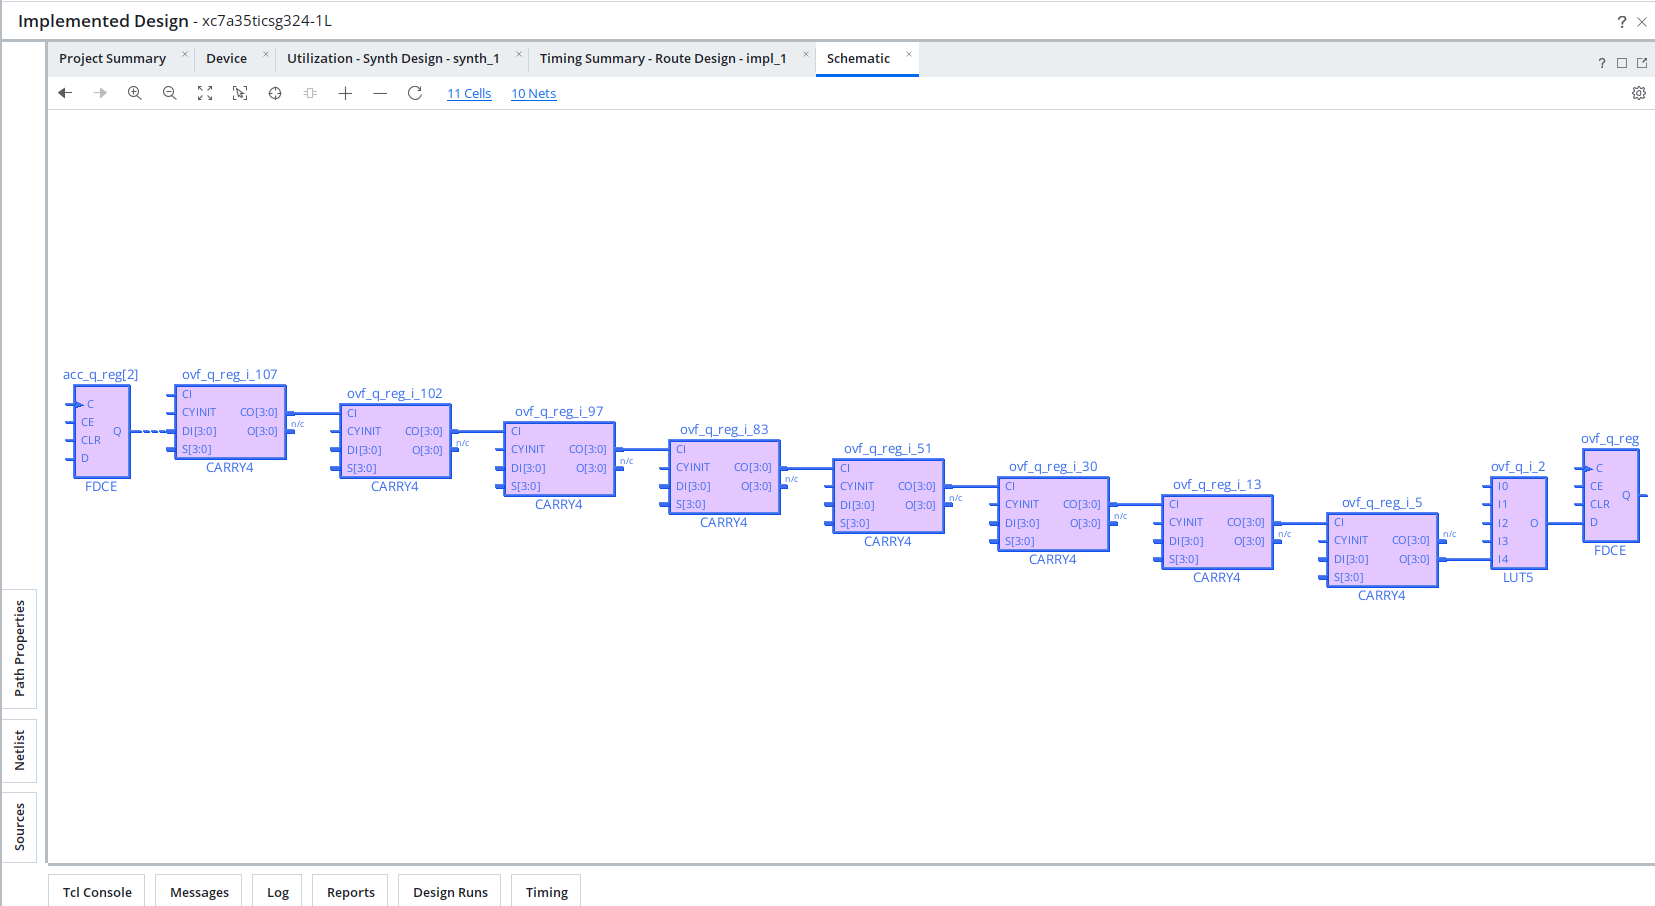
\includegraphics[width=0.95\linewidth]{critical-path.png}
    \caption{Artix-7 critical path: eight cascaded CARRY4 cells feeding a single LUT5 into the sticky overflow register.}
    \label{fig:critpath}
\end{figure}

The reason is structural. \texttt{acc\_ovf} compares the sign bits of
\texttt{acc\_q}, \texttt{product} and \texttt{sum}. Because it depends on
\texttt{sum}, it cannot begin evaluating until the entire carry chain has
resolved, and then needs a further one or two LUT levels on top. On the iCE40,
\texttt{acc\_q[31]} finishes with 1.8~ns more slack than \texttt{ovf\_q} does.

That two independent tools, from different vendors, targeting different
architectures at different process nodes, land on the same three gates is the
most instructive result in the project. Three gates that look free in the
source set $F_{max}$ on both parts, purely because they sit downstream of
everything else.

A sticky flag does not need to be correct in the cycle it is raised, which
suggests deferring the detection. That fix was measured rather than assumed;
Section~\ref{sec:defer} reports the result, including the fact that the obvious
form of it does not work.

\subsection{DSP48 Inference}
\label{sec:dsp}

A DSP48E1 is a $25\times18$ multiplier with a 48-bit accumulator, so an
$8\times8$ MAC with a 32-bit accumulator would appear to be an easy fit.
Vivado nonetheless maps the design entirely to LUTs and carry chains, and the
\texttt{(* use\_dsp = "yes" *)} attribute does not change this. Two properties
of the design prevent it:

\begin{enumerate}
    \item \textbf{The asynchronous reset.} No register inside a DSP48E1 has an
    asynchronous reset path, so \texttt{acc\_q} cannot be absorbed into one
    regardless of what the attribute requests.
    \item \textbf{The overflow detector.} \texttt{acc\_ovf} reads \texttt{sum},
    the adder output \emph{before} the register. Inside a DSP that node does not
    exist in the fabric, so the synthesiser would have to rebuild the entire
    32-bit adder in LUTs in any case --- at which point the hard block buys
    nothing.
\end{enumerate}

To confirm this rather than assert it, a stripped variant
(\texttt{synth/dsp\_experiment/mac\_core.v}) was written with both properties
removed: synchronous reset, no overflow detection, no rounding, no saturation.
It maps as textbook DSP48E1 accumulate mode, with \texttt{a} to $A[29{:}0]$,
\texttt{b} to $B[17{:}0]$, \texttt{acc\_q} to the block's internal P register,
\texttt{en} to \texttt{CEP}, and \texttt{!rst\_n || clear} to \texttt{RSTP} ---
which accounts for the single surviving LUT2. Ninety-seven LUTs, thirty-two
flip-flops and twenty-four carry chains collapse into one hard block.

\begin{figure}[H]
    \centering
    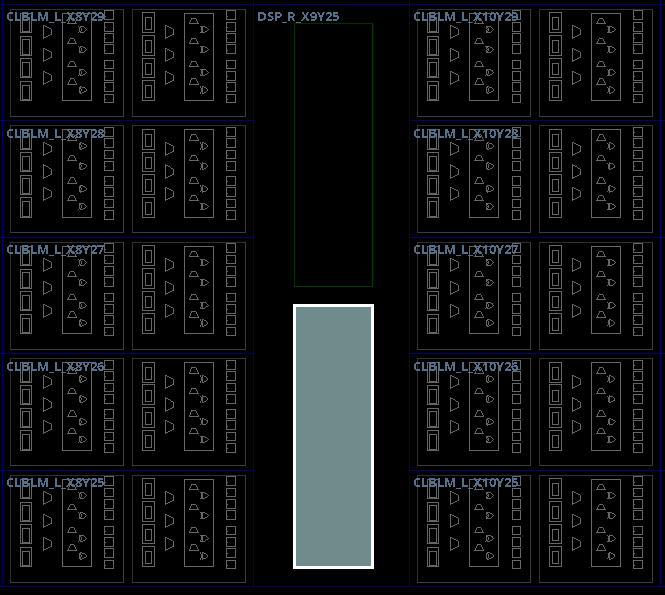
\includegraphics[width=0.75\linewidth]{dsp-device.png}
    \caption{The stripped variant placed and routed. The entire multiply-accumulate --- multiplier, 32-bit adder and accumulator register --- occupies the single shaded DSP48E1; the neighbouring DSP tile and the surrounding CLB columns are unused.}
    \label{fig:dspdevice}
\end{figure}

The $\leq 464.3$~MHz figure in Table~\ref{tab:artix} is a ceiling rather than a
measurement. With the accumulator inside the DSP there are no
register-to-register paths remaining in the fabric, so
\texttt{report\_timing\_summary} returns \texttt{inf} for worst negative slack
and \texttt{NA} for setup. The only remaining constraint is the block's own
pulse-width check: a \texttt{DSP48E1/CLK} minimum period of 2.154~ns. Adding
input registers would place real paths back under the timing engine at the cost
of a cycle of latency.

\subsection{Deferring Overflow Detection}
\label{sec:defer}

Section~\ref{sec:dsp} and the critical path above both indict the same three
gates, so the obvious remedy is to register \texttt{acc\_ovf} and OR it in a
cycle later. That does not work. The flag would still be computed from
\texttt{sum}, so \texttt{acc\_q} $\rightarrow$ carry chain $\rightarrow$ LUT
remains in the path; only the destination flip-flop changes.

Removing the path requires eliminating the dependency on \texttt{sum}
altogether. \texttt{synth/dsp\_experiment/mac\_ovf\_reg.v} latches the two
operand sign bits at the same edge the accumulator updates, then performs the
comparison one cycle later against the \emph{registered} accumulator:

\begin{lstlisting}[language=Verilog]
// at edge N: acc_q <= sum, sign_acc_q <= acc_q[MSB], sign_prd_q <= product[MSB]
wire ovf_detect = (sign_acc_q == sign_prd_q) &&
                  (acc_q[ACC_WIDTH-1] != sign_acc_q);
\end{lstlisting}

Every term is a flip-flop output, so the detector becomes
flop $\rightarrow$ one LUT $\rightarrow$ flop. Measured post-route under the
identical 5.000~ns constraint:

\begin{table}[H]
\centering
\caption{Effect of deferring overflow detection by one cycle}
\label{tab:defer}
\renewcommand{\arraystretch}{1.3}
\begin{tabular}{|l|c|c|c|c|}
\hline
 & \textbf{\texttt{mac}} & \textbf{\texttt{mac\_ovf\_reg}} & \textbf{Change} & \textbf{\texttt{mac\_core}} \\
\hline
LUTs        & 146       & 115       & $-31$ ($-21\%$) & 97 \\
Flip-flops  & 33        & 35        & $+2$            & 32 \\
CARRY4      & 35        & 27        & $-8$            & 24 \\
WNS         & 1.540 ns  & 2.195 ns  & $+0.655$ ns     & 2.187 ns \\
$F_{max}$   & 289.0 MHz & 356.5 MHz & $+67.5$ MHz     & 355.5 MHz \\
Path ends at & \texttt{ovf\_q} & \texttt{acc\_q[29]} & --- & \texttt{acc\_q[29]} \\
\hline
\end{tabular}
\end{table}

The new critical path is \texttt{acc\_q\_reg[1]} $\rightarrow$ one LUT3
$\rightarrow$ eight cascaded CARRY4 cells $\rightarrow$ \texttt{acc\_q\_reg[29]}:
the accumulator's own carry chain, with the overflow logic entirely absent. The
worst hold path is now \texttt{sign\_prd\_q\_reg} $\rightarrow$ \texttt{ovf\_q\_i\_1}
(a single LUT5) $\rightarrow$ \texttt{ovf\_q\_reg} at 0.259~ns, which is the
detector in its new, short form.

Two results are worth drawing out. First, at 356.5~MHz the deferred variant is
indistinguishable from \texttt{mac\_core} at 355.5~MHz. A datapath carrying full
overflow detection, rounding and saturation now runs as fast as a bare
multiply-accumulate carrying none of it; the 1~MHz difference is placement
noise. Both are limited by the same accumulator carry chain, which is the real
floor for this architecture.

Second, the variant is \emph{smaller} than the original by 31 LUTs and 8 carry
chains, paying only two flip-flops and one additional control set. Computing
overflow from \texttt{sum} obliged the synthesiser to build a 32-bit comparison
against a value that is itself the output of a 32-bit adder; reading three
registered bits instead collapses that to a single LUT5.

This is a synthesis measurement, not a drop-in replacement. Because
\texttt{overflow} now asserts one cycle after the operation that causes it,
\texttt{tb/tb\_mac.v} reports failures on its overflow-timing checks against
this variant. Adopting the structure in \texttt{rtl/mac.v} would mean updating
those expectations first, and the shipped unit deliberately still raises the
flag in the same cycle.

\subsection{Cost of Correctness per MAC in an Inference Array}

Comparing the first two rows of Table~\ref{tab:artix} isolates the price of the
numerical safeguards:

\begin{table}[H]
\centering
\caption{Cost of overflow detection, rounding and saturation on Artix-7}
\label{tab:cost}
\renewcommand{\arraystretch}{1.3}
\begin{tabular}{|l|c|c|c|}
\hline
\textbf{Metric} & \textbf{Bare MAC} & \textbf{Full unit} & \textbf{Deferred (\S\ref{sec:defer})} \\
\hline
LUTs        & 97        & 146 ($+49$)       & 115 ($+18$) \\
CARRY4      & 24        & 35 ($+11$)        & 27 ($+3$) \\
Flip-flops  & 32        & 33 ($+1$)         & 35 ($+3$) \\
$F_{max}$   & 355.5 MHz & 289.0 MHz ($-19\%$) & 356.5 MHz (no cost) \\
DSP48E1 mappable & Yes  & No        & No \\
\hline
\end{tabular}
\end{table}

On a part with hard multipliers the arithmetic is very nearly free --- one
DSP48E1 and a single LUT. Essentially all of the remaining logic is the
correctness guarantees wrapped around it, and those guarantees are also what
make the unit unmappable to the hard block in the first place.

The third column changes the reading of the second. The 49 LUTs and 66.5~MHz
are not what correctness costs; they are what correctness costs when it is
computed in the same cycle as the operation it describes. Given one cycle of
latency on the flag, the same guarantees cost 18 LUTs and no frequency at all.

This reframes the design question. For an inference accelerator the interesting
tradeoff is not ``LUT or DSP'' but which numerical guarantees are worth paying
for per MAC, given that a systolic array replicates the decision hundreds of
times. Saturation is cheap insurance against sign-flipped activations.
Per-MAC overflow detection may not be, if a single detector at the end of an
accumulation chain would serve --- a design the measurements here make
quantifiable rather than a matter of taste.

\subsection{Tool Observations}

Two non-obvious behaviours were encountered and are recorded because both
initially produced misleading results:

\begin{itemize}
    \item \textbf{\texttt{MAX\_DSP} is persistent.} In Vivado project mode,
    \texttt{MAX\_DSP} is a property of the synthesis run rather than a
    per-invocation flag. Setting it to zero once silently applies to every
    subsequent run in that project. Three runs were invalidated before this was
    identified.
    \item \textbf{\texttt{use\_dsp} is a hint.} The attribute requests DSP
    inference; it does not compel it. When the structure cannot map, Vivado
    declines silently and reports zero DSPs with no warning.
\end{itemize}

%-----------------------------------------------------------
\section{Hardware Demonstration}
%-----------------------------------------------------------

\texttt{rtl/mac\_top.v} wraps the unit for the Nandland Go Board
(iCE40HX1K-VQ100, 25~MHz). An eight-entry ROM of Q1.7 operand pairs is stepped
by a debounced push-button, and the scaled output is displayed in hexadecimal
on the two seven-segment digits. The sequence is chosen to walk through every
behaviour of interest, including both saturation directions.

\begin{table}[H]
\centering
\caption{Operand ROM and expected display after each button press}
\label{tab:rom}
\renewcommand{\arraystretch}{1.3}
\begin{tabular}{|c|r|r|r|r|c|l|}
\hline
\textbf{\#} & \textbf{$a$} & \textbf{$b$} & \textbf{product} & \textbf{running acc} & \textbf{display} & \textbf{behaviour} \\
\hline
0 & 64    & 64  & $+0.250$ & $0.250$  & \texttt{20} & plain accumulate \\
1 & 64    & 64  & $+0.250$ & $0.500$  & \texttt{40} & \\
2 & 64    & 64  & $+0.250$ & $0.750$  & \texttt{60} & \\
3 & 64    & 64  & $+0.250$ & $1.000$  & \texttt{7F} & saturates high, LED1 on \\
4 & $-64$ & 127 & $-0.496$ & $0.504$  & \texttt{41} & returns in range \\
5 & $-128$& 127 & $-0.992$ & $-0.488$ & \texttt{C2} & negative result \\
6 & $-128$& 127 & $-0.992$ & $-1.480$ & \texttt{80} & saturates low \\
7 & 0     & 0   & $0$      & $-1.480$ & \texttt{80} & enable with zero operands \\
\hline
\end{tabular}
\end{table}

\begin{figure}[H]
    \centering
    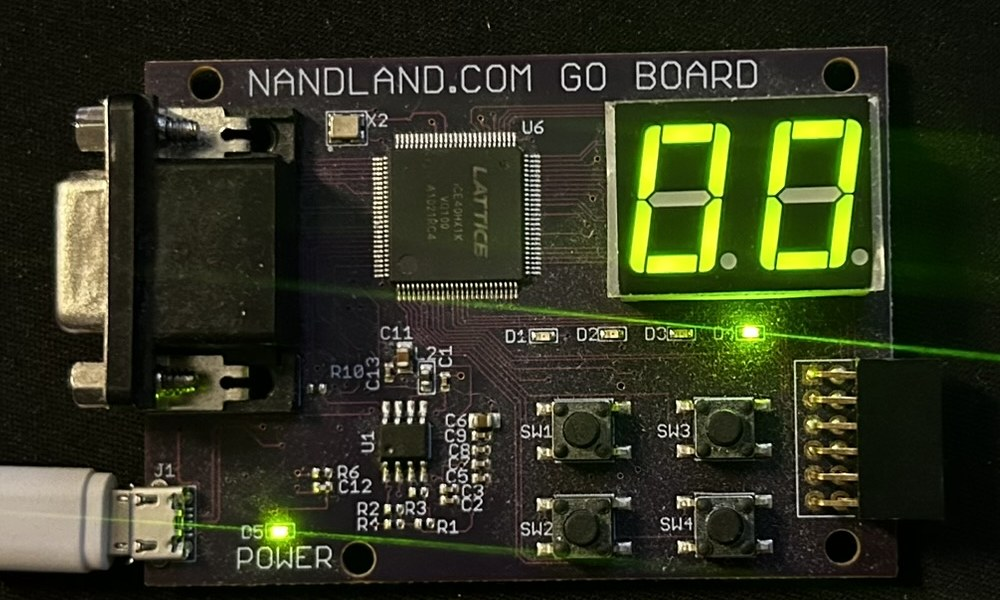
\includegraphics[width=0.7\linewidth]{board.jpg}
    \caption{The MAC unit running on the Nandland Go Board. LED~4 is the heartbeat; the display shows the scaled Q1.7 result in hexadecimal.}
    \label{fig:board}
\end{figure}

\begin{figure}[H]
    \centering
    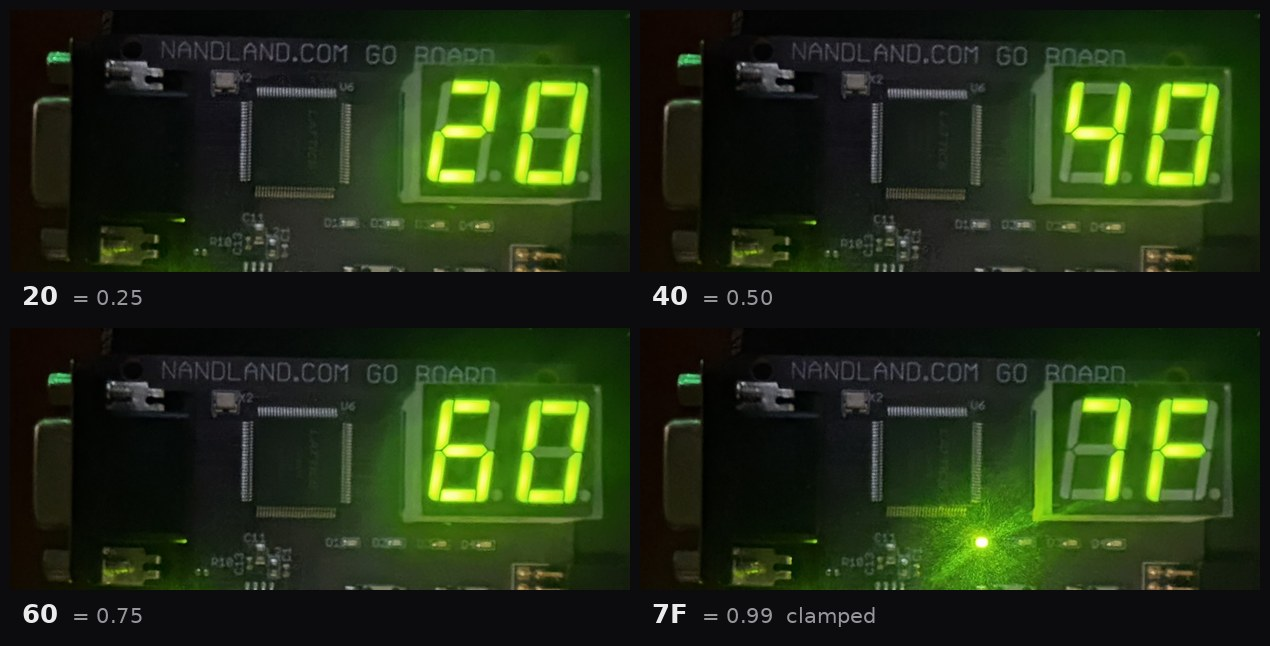
\includegraphics[width=0.85\linewidth]{sequence.jpg}
    \caption{Four successive presses of the step button: \texttt{20}, \texttt{40}, \texttt{60}, \texttt{7F}. The fourth saturates, matching row 3 of Table~\ref{tab:rom}.}
    \label{fig:sequence}
\end{figure}

All fourteen observed board values were checked against independently computed
arithmetic and matched exactly. Switch~2 clears the accumulator and rewinds the
ROM, Switch~3 is reset, and Switch~4 displays \texttt{acc[7:0]} instead of the
scaled result. LED~4 is a heartbeat driven from bit~23 of a free-running
counter, which confirms the bitstream loaded and the board is clocking
independently of whether the design is behaving.

The accumulator is deliberately not brought out to pins in this wrapper.
Exposing all 32 bits consumes 62 of the 72 available I/O and fills three of the
four I/O banks, leaving nothing for the LEDs and display --- acceptable for a
synthesis measurement, but not for a board demonstration.

%-----------------------------------------------------------
\section{Conclusion and Remarks}
%-----------------------------------------------------------

A parameterised signed fixed-point multiply-accumulate unit was designed,
verified and characterised across two FPGA families. All stated objectives were
met: the unit performs one MAC per cycle, is genuinely parameterised across
four verified configurations, rounds to nearest, saturates rather than wraps,
detects accumulator overflow with a sticky flag, and runs on physical hardware
with every displayed value matching hand-computed arithmetic.

Timing closed at 132.64~MHz on iCE40HX1K and 289.0~MHz on Artix-7
XC7A35T-1L, both post-route, from identical Verilog-2001 source.

Three results are worth restating. First, the critical path terminates at the
sticky overflow flag on both devices --- two vendors, two architectures, two
independent timing engines, one bottleneck, and one predicted in the source
comments before it was measured. Second, the design will not map to a DSP48E1,
for reasons that were measured and isolated rather than assumed. Third, and
following from the second, the numerical correctness logic costs 49 LUTs and
19\% of maximum frequency, and is precisely what prevents the hard block from
being used --- which makes ``how much correctness per MAC'' a quantified design
decision rather than a stylistic one.

The immediate extension is a $4\times4$ systolic array: sixteen of these units
in a grid with operands flowing left-to-right and weights top-to-bottom, which
is how a matrix engine is actually built. \texttt{mac.v} is parameterised and
drops in unchanged.

\end{document}
